\section*{Abstract}

Our project is a survival game called \textbf{Maze Escape}. The goal of the project is to show the practical use of artificial intelligence search algorithms and machine learning. The game simulates humans being chased by monsters on a $30 \times 30$ toroidal grid map (wrapping edges). The system uses and compares five AI search strategies: \textbf{A* pathfinding}, \textbf{Greedy Algorithm}, \textbf{breadth-first search (BFS)}, \textbf{Minimax Algorithm}, and \textbf{Simulated Annealing Algorithm}. The maze is generated by a \textbf{Genetic Algorithm (GA)}. The GA improves map connectivity, wall density, path diversity, and branch structure through multi-generation evolution.

This project shows how artificial intelligence behaves under limited, competitive, and real-time conditions. It also shows how different search strategies change the difficulty of the game and affect the player experience. The A* algorithm creates the most direct pursuit path. The greedy algorithm gives fast performance with low computing cost. The simulated annealing algorithm adds controlled randomness and makes monster movement less predictable. The genetic algorithm keeps generating connected and navigable maps to maintain gameplay quality. With the addition of machine learning, interceptors can scroll to predict the position of the next three human steps, thus blocking possible escape routes.

\section{Introduction}
\begin{figure}[htbp]
    \centering
    \IfFileExists{system.png}{
        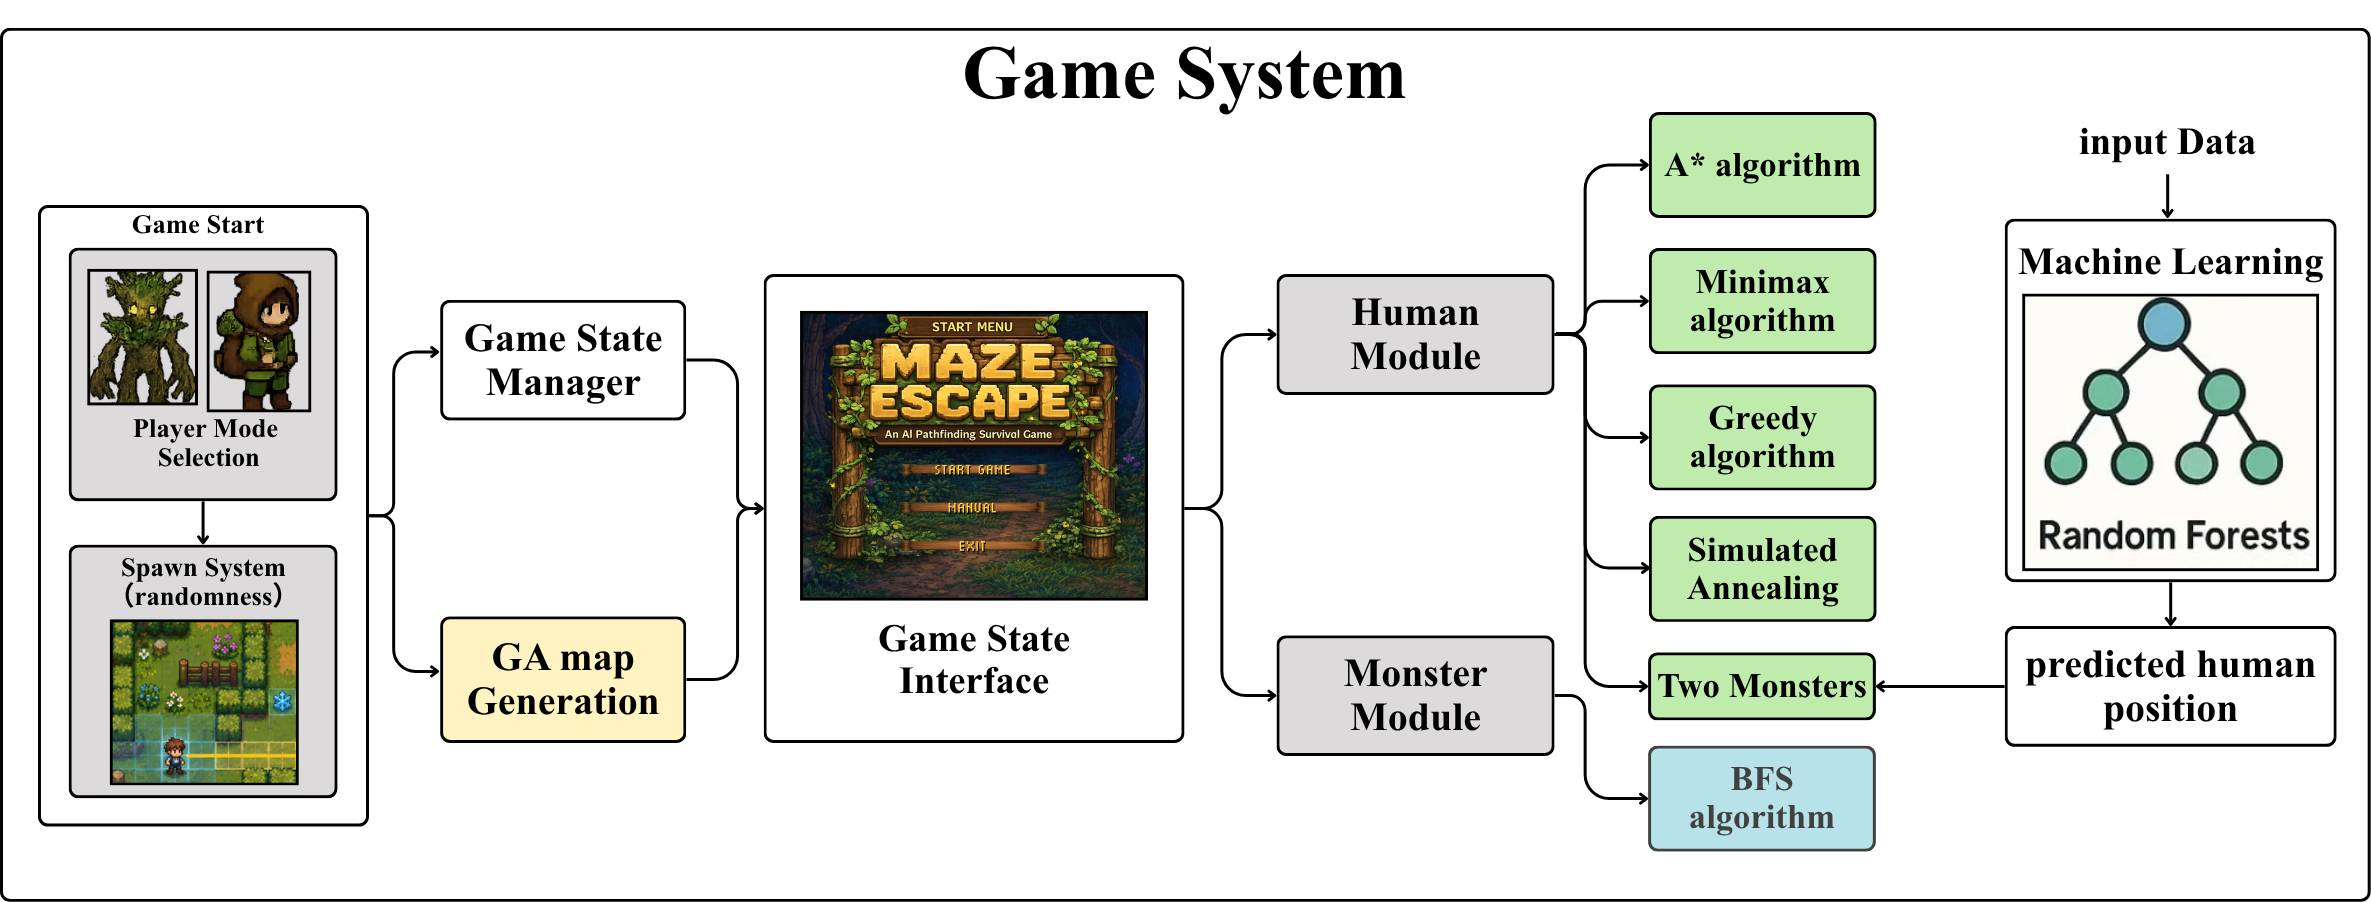
\includegraphics[width=0.8\textwidth]{system.png}
    }{
        \fbox{\parbox[c][4cm][c]{0.75\textwidth}{
            \centering Missing image: \texttt{system.png}
        }}
    }
    \caption{Game System}
    \label{fig:example}
\end{figure}

In the course ``Principles of Artificial Intelligence,'' we studied a variety of search, planning, and optimization algorithms. Based on these core methodologies, our Maze Escape project extends static, single-agent pathfinding into dynamic, multi-dimensional adversarial scenarios. To achieve this transition, we introduce randomly generated maze maps based on genetic algorithms, expand the dimensional space, and a two-way tracking mechanism enhanced by predictive machine learning has been realized.

In order to comprehensively evaluate these algorithms, we have designed two complementary game modes: escape mode and chase mode. In the chase mode, the actions of human characters are driven by evasion algorithms based on Breadth-First Search (BFS). For the core task of predators pursuing prey, the project adopts four distinct intelligent strategies and combined with machine learning-driven interception mechanism:

\begin{itemize}
    \item \textbf{A* Search Algorithm:} In single-monster mode, the algorithm calculates the shortest path to the player. In dual-monster mode, monsters are divided into two types: direct pursuers and interceptors. The interceptors predict the player's next move and block potential escape routes.

    \item \textbf{Greedy Algorithm:} It calculates a distance field centered at the player's current position, causing monsters to always move toward the nearest neighboring node. This pursuit method is highly efficient and requires low computational resources.

    \item \textbf{Minimax Decision Tree:} This strategy treats the pursuit process as a two-player zero-sum game. The algorithm combines $\alpha$-$\beta$ pruning with a transposition table to predict subsequent moves. The monster aims to minimize the player's safety score during the game, while simultaneously simulating the player's efforts to maximize it, thereby enabling efficient pursuit from both perspectives.

    \item \textbf{Simulated Annealing Algorithm:} The algorithm first generates an initial movement path and then randomly adjusts it through repeated iterations. Following the cooling schedule, the system accepts suboptimal moves with a certain probability, making the monster's actions more stochastic and harder to predict.

    \item \textbf{Machine Learning:} Based on spatial characteristics (the relative position of humans relative to monsters, local wall obstacles and the direction of movement of the first two steps), we have trained a random forest model to predict the next move of human players, and predict the position of the next three steps by rolling, so as to achieve effective blockade.
    
\end{itemize}

The core environment of our project is a $30 \times 30$ toroidal grid map, where the maze layouts are generated by a highly customized Genetic Algorithm (GA). The algorithm maintains a population of candidate maps and evolves them for more than 20 generations. The fitness function balances several critical factors, including strong floor connectivity, approximately 28\% wall density, a high number of three-way and four-way junctions, and an average BFS path length close to 20 steps between randomly selected positions. The system also utilizes tournament selection, row-and-column crossover, and bit-flip mutation. These methods effectively assist the algorithm in generating maps with high accessibility, spatial diversity, and appropriate difficulty.

The following sections of this report will introduce the design and specific implementation methods of each component in detail, quantitatively analyze the algorithmic characteristics of each AI strategy along with its impact on gameplay, and reflect on their respective advantages and limitations observed during the development process.
